\documentclass[11pt]{article}
\usepackage[utf8]{inputenc}
\usepackage[nottoc,numbib]{tocbibind}
\usepackage[parfill]{parskip}
\usepackage{graphicx}
\usepackage[justification=centering]{caption}
\usepackage{float}
\usepackage[sort,numbers]{natbib}
\usepackage{array}
\usepackage{longtable}
\usepackage[skip=5pt]{caption}
\usepackage{mathtools}
\usepackage[toc,page]{appendix}
\usepackage{subcaption}
\usepackage[swedish,english]{babel}
\usepackage{pdfpages}
\usepackage{booktabs}
\usepackage{changepage}

\newcolumntype{L}[1]{>{\raggedright\let\newline\\\arraybackslash\hspace{0pt}}m{#1}}
\newcolumntype{C}[1]{>{\centering\let\newline\\\arraybackslash\hspace{0pt}}m{#1}}
\newcolumntype{R}[1]{>{\raggedleft\let\newline\\\arraybackslash\hspace{0pt}}m{#1}}

\makeatletter
\newcommand*{\centerfloat}{%
  \parindent \z@
  \leftskip \z@ \@plus 1fil \@minus \textwidth
  \rightskip\leftskip
  \parfillskip \z@skip}
\makeatother

\begin{document}

\pagenumbering{gobble}

\title{Identifying pathogenic amino acid substitutions in human proteins using deep learning}
\date{April 30, 2018}
\author{Alexander Kvist}

%%%%%%%%
\pagenumbering{gobble}
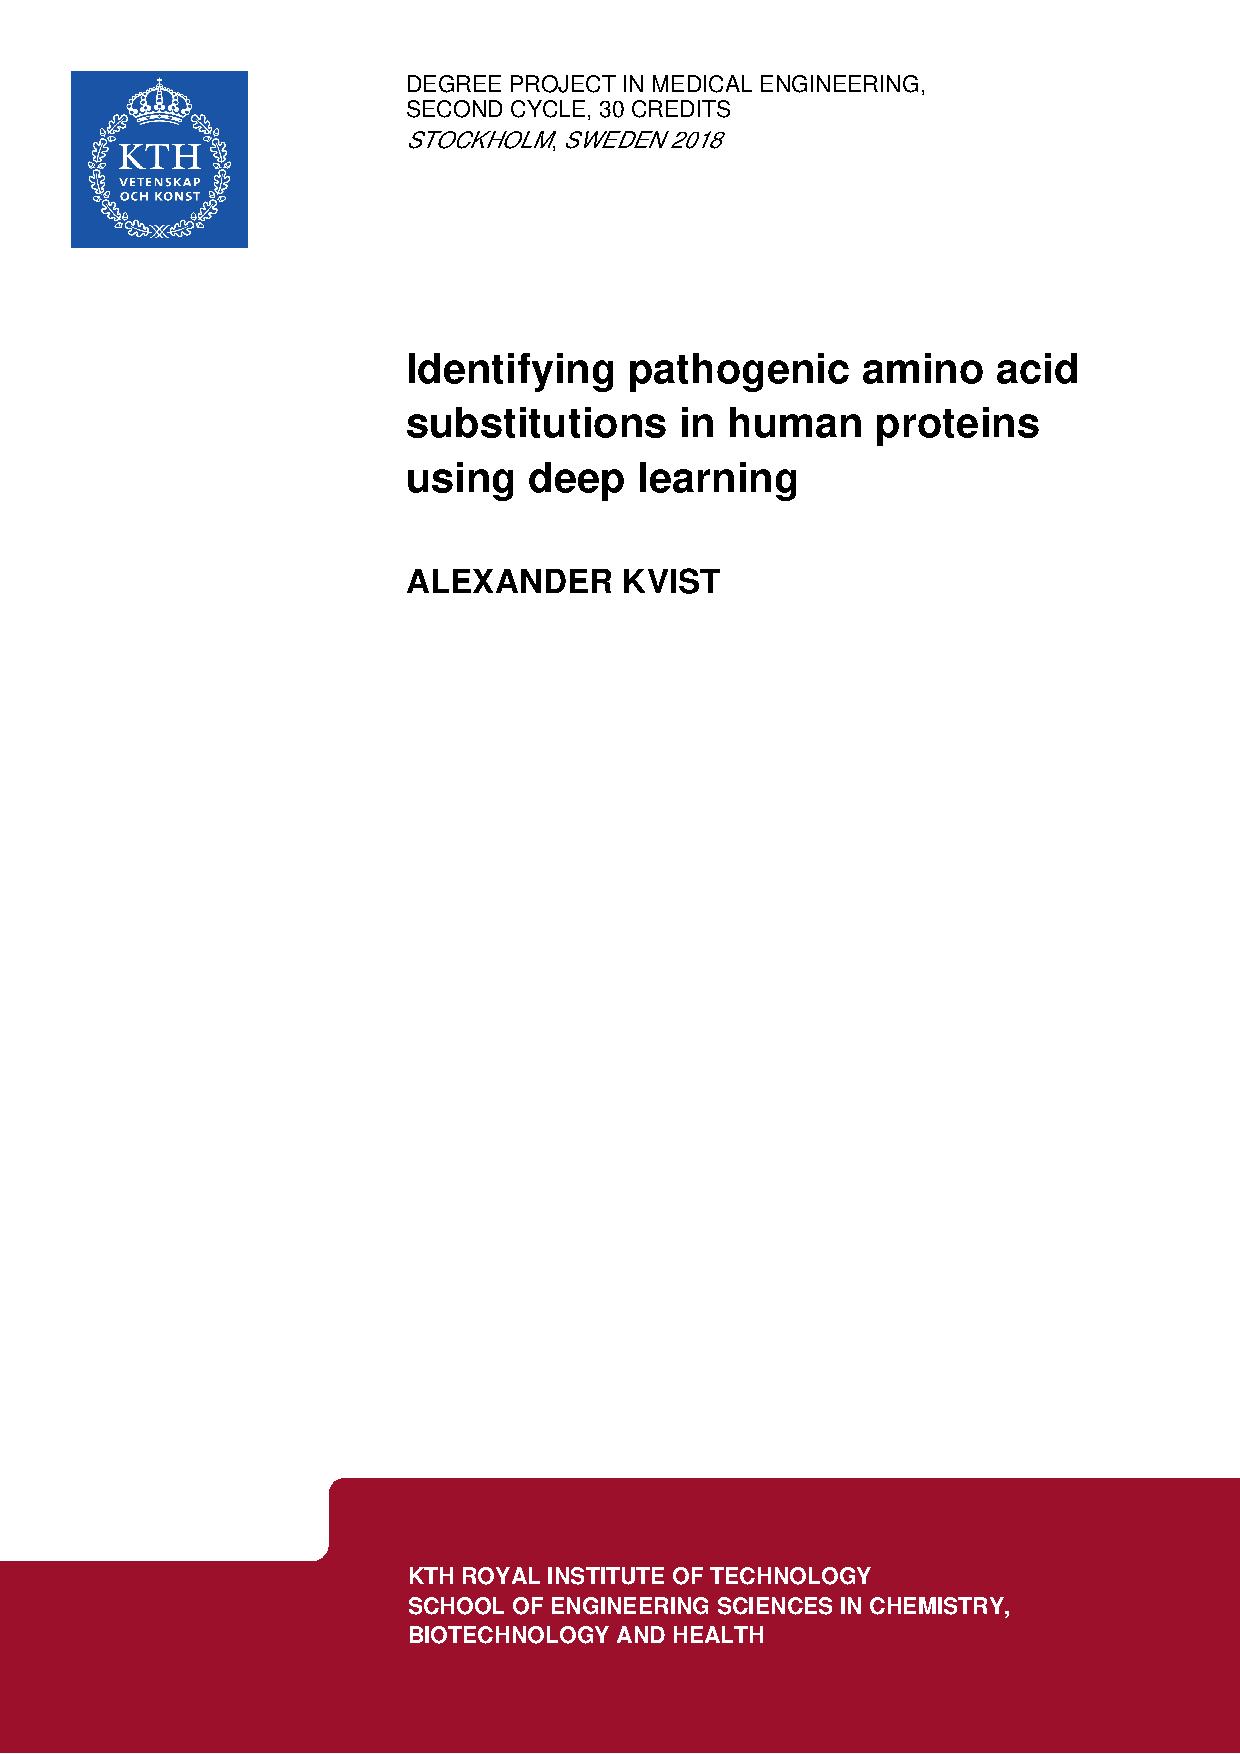
\includepdf[pages={1}]{omslag_baksida.pdf}
\newpage
\mbox{}
\newpage
\pagenumbering{roman}

\selectlanguage{english}
\begin{abstract}

Many diseases of genetic origin originate from non-synonymous single nucleotide polymorphisms (nsSNPs). These cause changes in the final protein product encoded by a gene. Through large scale sequencing and population studies, there is growing availability of information of which variations are tolerated and which are not. Variant effect predictors use a wide range of information about such variations to predict their effect, often focusing on evolutionary information. Here, a novel amino acid substitution variant effect predictor is developed. The predictor is a deep convolutional neural network incorporating evolutionary information, sequence information, as well as structural information, to predict both the pathogenicity as well as the severity of amino acid substitutions. The model achieves state-of-the-art performance on benchmark datasets.

\end{abstract}
\newpage
\thispagestyle{empty}
\mbox{}
\newpage
%%%%%%%

\tableofcontents{}
\clearpage

\newpage
\thispagestyle{empty}
\mbox{}
\newpage

\pagenumbering{arabic}

\section{Introduction}

With increasing availability of genome and proteome data through advances in sequencing technology, more genetic variants are discovered at an increasing rate. Many diseases arise from non-synonymous single nucleotide polymorphisms (nsSNPs), resulting in amino acid substitutions in encoded protein products. While not all amino acid substitutions are harmful, certain substitutions can impede critical protein function by effects such as abnormal folding or how the protein is post-translationally modified\cite{niroula2016variation}.
Establishing the effect of amino acid substitutions experimentally can be time consuming, so computational variant effect predictions are important both as a source of evidence for interpretation, and as a sorting step for choosing which mutations to study further.

%databases
A number of databases exist for curating variants and experimentally verified effects. Often these are locus-specific databases (LSDBs), focused on certain genes or diseases. Recently, efforts also exist for creating standard benchmark databases for creation and benchmarking of computational effect prediction tools. One example is the VariBench\cite{nair2013varibench} database, containing datasets with both positive and negative examples of variations, such as disease-causing mutations and neutral mutations frequently found in healthy individuals.

Several computational tools have been developed for assessing the functional impact of nsSNPs and other forms of mutations. Some tools are more specialized than others, with some designed to predict cancer variants\cite{reva2011predicting} or to predict effects in specific proteins\cite{niroula2015classification}. 

Commonly these tools are based on some form of analysis based on protein sequence, sequence homology, protein structure analysis, sequence annotations, or physiochemical properties of amino acids involved in the mutation\cite{ng2006predicting}. For example, a tool used for assessing if an amino acid substitution has an effect on protein function, SIFT, does this by analyzing the conservation value of amino acid positions in an alignment of homologous protein sequences\cite{kumar2009predicting}. Other tools using machine learning methods trained on disease-causing variants implement biochemical properties of amino acids in addition to evolutionary information in order to predict pathogenic variants\cite{niroula2015pon}. A recent predictor developed by Niroula et al\cite{niroula2017predicting} has been used to assign a disease severity score for amino acid substitutions. The tool, PON-PS, does this by feeding a number of features such as selective pressure and properties of amino acids into a random forest algorithm. It allows for prediction of the disease severity of novel variants, since the predictor is trained on a large number of different proteins.

Recently, deep learning methods have shown promise in predicting protein properties.
Elofsson Lab has used deep learning methods to predict protein contacts and for improving protein model quality assessment\cite{skwark2014improved}\cite{uziela2017proq3d}. A deep learning approach allows for utilising low level information such as the amino acid sequence itself to extract relevant features, and the methods show high prediction accuracy. The deep learning approach used to predict structural properties of proteins could also be of use in identifying disease-causing amino acid substitutions.

\section{Materials and Methods}

\subsection{Datasets}

Four different datasets are used for training and testing prediction models. The datasets used are summarized in Table \ref{table:datasets_tolerance} and Table \ref{table:dataset_severity}. 
The first dataset is a benchmark dataset from the VariBench\cite{nair2013varibench} database, used to train and test PON-P2\cite{niroula2015pon}. The dataset contains pathogenic variants in the form of disease-causing missense variations along with neutral variants in the form of common polymorphisms. It contains 13885 pathogenic variants and 14674 neutral variants from 1073 and 6602 proteins, respectively. The dataset comes from a larger dataset from which cancer cases are filtered, since such variants are thought to have different working mechanisms and patterns.

Two more datasets are obtained from the website of PolyPhen-2\cite{PolyPhen-2data}: HumDiv and HumVar, both compiled from variants found in the UniProtKB database. HumDiv contains Mendelian disease variants with known effects on molecular function, along with neutral variants. It contains 5564 deleterious and 7539 neutral variants from the same set of 978 human proteins. HumVar is composed of all human variants annotated with disease associations (filtered to exclude cancer cases), and neutral variants (common polymorphisms with minor allele frequency more than 1\%, without any reported disease associations). In total, it contains 22196 deleterious and 21151 neutral variants from 9679 human proteins.

An additional dataset containing phenotypic severity annotated disease variants is obtained from the VariBench database. These are variants obtained through data mining of literature and variant databases\cite{niroula2017predicting}. In total, this dataset contains 1028 mild, 501 moderate, and 1399 severe disease variants from 91 human proteins.

All datasets are split up into training and test sets. The VariBench datasets are downloaded in separate training and test sets, with variations in the same proteins located in either training or test sets. HumDiv and HumVar are split into 80/20\% training/test. The training sets are then further divided into training and validation sets. Around 20\% of the variants in the training sets are used as validation data. For the VariBench tolerance dataset, the training set is split such that there is no overlap between the proteins from which the variants are found in between training and validation, to better estimate when the model fails to generalize to other proteins.

\begin{table}
\caption{Source datasets for pathogenicity prediction}
\label{table:datasets_tolerance}
\begin{center}
\centerfloat
\begin{tabular}{lllllll}
\toprule
Dataset & Neutral variants & Pathogenic variants & Total variants & Proteins \\ 
\midrule
VariBench Tolerance & 14674 & 13885 & 28559 & 7675   \\ 
HumVar & 21151 & 22196 & 43347 & 9679   \\
HumDiv & 7539 & 5564 & 13103 & 978  \\ 
\bottomrule
\end{tabular}
\end{center}
\end{table}

\begin{table}
\caption{Source datasets for severity prediction}
\label{table:dataset_severity}
\begin{center}
\centerfloat
\begin{tabular}{lllllll}
\toprule
Dataset & Mild variants & Moderate variants & Severe variants & Total variants & Proteins \\ 
\midrule
VariBench Severity & 1028 & 501 & 1399 & 2928 & 91   \\ 
\bottomrule
\end{tabular}
\end{center}
\end{table}

\subsection{Features}

%We should insert a table of input features used 

For each variant, a number of features are extracted in order to describe it. These are obtained from the mutation, the protein sequence itself, annotations, as well as from a multiple sequence alignment (MSA) of homologous protein sequences. 22 characters are used to describe amino acids, as well as an extra character for gaps in alignments.

Protein homologues are found using protein BLAST against the NCBI nr database, with an E-value cutoff of 0.001. The homologues are then divided into two blocks, one containing sequences with sequence identity of 90\% or more to the reference sequence, and the other containing sequences with sequence identity below 90\% to the reference sequence. Sequences are then aligned into MSAs (one for each identity range) using MAFFT\cite{katoh2013mafft} with default parameters. From the MSAs, several statistics are calculated for a window of 10 amino acids in each direction from the mutation position. These are the frequencies of each amino acid and gap character for a position in the MSA along with the Shannon entropy (equation \ref{eq:shannon}), as well as the self-information (equation \ref{eq:self_info}) and partial entropy (equation \ref{eq:part_entr}) for each amino acid and gap character at a position:

\begin{equation} \label{eq:shannon}
S = -\sum_{i}^{K} p_i \log_2 p_i
\end{equation}

\begin{equation} \label{eq:self_info}
I_i = -log(\frac{p_i}{\bar{p_i}})
\end{equation}

\begin{equation} \label{eq:part_entr}
S_i = -p_i log(\frac{p_i}{\bar{p_i}})
\end{equation}

where K is the number of amino acid types, $p_i$ is the frequency of amino acid \textit{i} at a position, and $\bar{p_i}$ is the average frequency of amino acid \textit{i} over the Uniref50 database.

Furthermore, the amino acid sequence in the window is included by encoding each amino acid in a one-hot vector of length 22. Original and mutated residues are also encoded in a vector of length 44. To this vector is also appended a log-odds score (equation \ref{eq:lr_sum}) built from Gene Ontology (GO) terms. For each protein present in the training set associated with neutral or pathogenic variants, all GO terms associated with the protein were extracted from UniProtKB. All ancestors for the GO term were then collected using GOAtools\cite{tang2015goatools}. The frequencies of occurrence of each term were then calculated for pathogenic and neutral variants. The log-odds score is then calculated as:

\begin{equation} \label{eq:lr_sum}
LGO = \sum\log\frac{f(P_i)+1}{{f(N_i)+1}}
\end{equation}

where $f(P_i)$ is the frequency of the $i^{th}$ GO term in the pathogenic training set, and $f(N_i)$ is the frequency of the $i^{th}$ GO term in the neutral training set. For the VariBench severity dataset, $f(P_i)$ is calculated for severe variants, and $f(N_i)$ for mild and moderate variants together.

Structural information is also obtained by feeding the self-information, partial entropy, and amino acid sequence into a pre-trained deep convolutional neural network model developed for predicting certain structural properties for use in model quality assessment\cite{hurtado2018deep}. The self-information and partial entropy come from the alignment with 90\% or less sequence identity to reference sequence. The pre-trained model can be seen in Figure \ref{fig:ssmodel}. For each residue in the window, features obtained from this model are secondary structure in 3-state and 6-state representations, relative surface area, as well as the sine and cosine of the $\phi$ and $\psi$ protein backbone torsion angles\cite{xue2008real}. A summary of these features can be found in Table \ref{table:features}.

\begin{table}
\caption{Input features}
\label{table:features}
\begin{center}
\centerfloat
\begin{tabular}{lllllll}
\toprule
Feature & Dimensionality & Source \\ 
\midrule
Frequencies + Shannon entropy & 21x48 & MSA, both ranges    \\ 
Self-information & 21x46 & MSA, both ranges \\
Partial entropy & 21x46 & MSA, both ranges  \\ 
Sequence & 21x22 & Protein sequence  \\ 
Structural & 21x14 & Predicted using sequence and low range MSA  \\ 
Mutation and LGO & 1x45 & Mutation and GO annotations  \\ 
\bottomrule
\end{tabular}
\end{center}
\end{table}

\begin{figure}
  \centering
  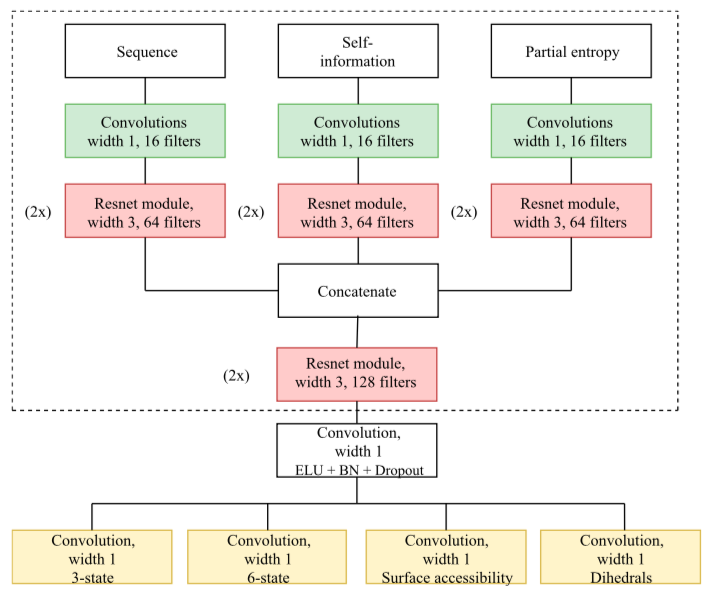
\includegraphics[scale=0.5]
    {ss_model.png}
  \centering
  \caption{ Pre-trained model for extracting structural information. Reproduced from Hurtado et al, 2018.\cite{hurtado2018deep} }
  \label{fig:ssmodel}
\end{figure}


\subsection{Model}

The developed model is a deep convolutional neural network using one-dimensional ResNet blocks. The ResNet block structure can be seen in Figure \ref{fig:block} and the model in Figure \ref{fig:model}. For each type of input calculated for the 21-residue window (frequencies, self-information, entropies, sequence, structural), a convolution of width 1 projects each input into a 21x32-dimensional space. This is followed by a number of ResNet blocks. These are then concatenated, followed by another number of ResNet blocks. The one-dimensional input is passed through its own branch. Branches are then concatenated, flattened, and end in a fully-connected layer of 128 neurons and a fully-connected sigmoid output layer for binary predictions of pathogenic or neutral variants, and for binary predictions of severe or non-severe variants. For multi-class classification, the output layer is composed of three neurons with softmax activation. Due to the small size of the severity dataset, the model for severity prediction has weights initialized from a model trained for pathogenicity prediction on the VariBench tolerance dataset and is then re-trained on the severity dataset.

The models are built using Keras\cite{chollet2015keras}, and training is guided by the Adam\cite{kingma2014adam} optimizer. For binary prediction, the loss function is binary cross-entropy, and for multi-class prediction, the loss function is categorical cross-entropy. Hyperparameters are optimized using the validation sets, taking into consideration validation loss as well as metrics evaluated on the validation sets after training. Early stopping is implemented during training. A grid search over dropout values and depth of ResNet blocks for the VariBench tolerance dataset resulted in a dropout of 0.7 and a depth of 6 blocks.

To gain an idea of what type of inputs contribute to performance, three additional versions of the model with branches excluded or modified were also evaluated on the VariBench tolerance dataset. These include a model with the structural input branch removed, a model with GO term removed, and a model not relying on any input from alignments. For the non-alignment model, self-information and partial entropy branches were dropped, and the frequency branch was replaced with BLOSUM62 substitution matrix scores for each type of amino acid in the 21-residue window. A version of the pre-trained model for extracting structural features using only sequence as input was used for obtaining input to the structural branch. The substitution score between original and altered amino acid in the BLOSUM62 matrix was also appended to the one-dimensional input in this model.

\begin{figure}[h!]
  \centering
  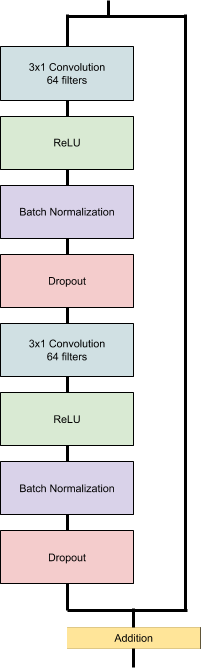
\includegraphics[scale=0.3]
    {Block_cropped.png}
  \centering
  \caption{ ResNet block structure }
  \label{fig:block}
\end{figure}

\begin{figure}[h!]
\hspace*{-0.8in}
  \centering
  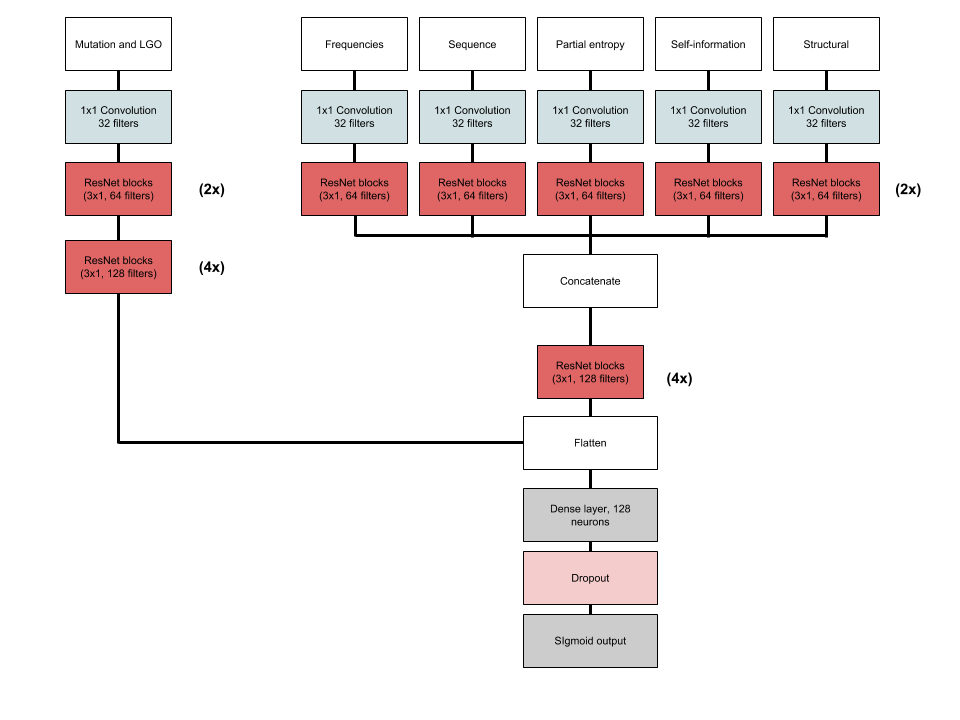
\includegraphics[scale=0.5]
    {model.png}
  \centering
  \caption{ Model architecture }
  \label{fig:model}
\end{figure}

\subsection{Evaluation metrics}

To obtain a robust evaluation of the model's prediction accuracy, a number of statistics are calculated. These are positive predictive value (PPV), negative predictive value (NPV), Sensitivity, Specificity, Accuracy, and Matthews Correlation Coefficient (MCC). These measures are calculated as:

\begin{equation} \label{eq:ppv}
PPV = \frac{TP}{{TP+FP}}
\end{equation}

\begin{equation} \label{eq:npv}
NPV = \frac{TN}{{TN+FN}}
\end{equation}

\begin{equation} \label{eq:sens}
Sensitivity = \frac{TP}{{TP+FN}}
\end{equation}

\begin{equation} \label{eq:spec}
Specificity = \frac{TN}{{TN+FP}}
\end{equation}

\begin{equation} \label{eq:acc}
Accuracy = \frac{TP+TN}{{TP+TN+FP+FN}}
\end{equation}

\begin{equation} \label{eq:mcc}
MCC = \frac{TP*TN - FP*FN}{{\sqrt{(TP+FP)(TP+FN)(TN+FP)(TN+FN)}}}
\end{equation}

where TN and TP are true negatives and positives, and FN and FP are false negatives and positives.

For binary predictions, the receiver operating characteristic (ROC) curve and the area under curve (AUC) are calculated, as well as a precision-recall curve (PRC). For the 3-class severity predictions, a confusion matrix is shown.


\section{Results}
    
\subsection{VariBench tolerance}

The reported performances for the VariBench tolerance dataset found in literature\cite{niroula2015pon} along with those of the developed model can be seen in Table \ref{table:varibench_tolerance_val} and Table \ref{table:varibench_tolerance_test}. Note that the performance measures noted as \textit{confident} were reported only for variants which the predictor was confident on, disregarding difficult or unreliable cases (about 40\% of variants\cite{niroula2015pon}). For predicting on all variants, the developed model has higher performance than previous methods with reported performances.

The performance of different versions of the developed model on the independent test set can be seen in Table \ref{table:model_versions}. Performance can be seen to only drop marginally when the structural branch is removed, while the drop is more significant for the non-alignment model and the model not using GO terms.

\begin{table}
\caption{Performance of model versions on test set}
\label{table:model_versions}
\begin{center}
\begin{tabular}{lllllll}
\toprule
Model version & PPV & NPV & Sens & Spec & Acc & MCC\\ 
\midrule
Full model & 0.75 & 0.87 & 0.85 & 0.78 & 0.81 & 0.62   \\
Structural input removed & 0.74 & 0.83 & 0.80 & 0.78 & 0.79 & 0.58  \\ 
Non-alignment model & 0.75 & 0.77 & 0.69 & 0.81 & 0.75 & 0.51   \\
GO term removed & 0.71 & 0.78 & 0.72 & 0.77 & 0.75 & 0.50  \\ 
\bottomrule
\end{tabular}
\end{center}
\end{table}


\begin{table}
\caption{Metrics on VariBench tolerance dataset: validation}
\label{table:varibench_tolerance_val}
\begin{center}
\begin{tabular}{lllllll}
\toprule
Predictor & PPV & NPV & Sens & Spec & Acc & MCC\\ 
\midrule
\textbf{Developed model} & 0.85 & 0.83 & 0.85 & 0.82 & 0.84 & 0.67   \\ 
PON-P2 (confident) & \textit{0.89} & \textit{0.91} & \textit{0.89} & \textit{0.91} & \textit{0.90} & \textit{0.80}   \\ 
PON-P (confident) & \textit{0.87} & \textit{0.87} & \textit{0.88} & \textit{0.85} & \textit{0.87} & \textit{0.73}  \\ 
PON-P2 (all) & 0.80 & 0.82 & 0.81 & 0.81 & 0.81 & 0.62   \\
Condel & 0.75 & 0.75 & 0.77 & 0.73 & 0.75 & 0.50   \\
PolyPhen-2 & 0.72 & 0.79 & 0.83 & 0.66 & 0.75 & 0.50  \\ 
Provean & 0.72 & 0.79 & 0.81 & 0.70 & 0.75 & 0.51   \\
SIFT & 0.71 & 0.78 & 0.79 & 0.70 & 0.74 & 0.48  \\ 
SNAP & 0.70 & 0.78 & 0.81 & 0.67 & 0.74 & 0.48  \\
\bottomrule
\end{tabular}
\end{center}
\end{table}

\begin{table}
\caption{Metrics on VariBench tolerance dataset: separate test set}
\label{table:varibench_tolerance_test}
\begin{center}
\begin{tabular}{lllllll}
\toprule
Predictor & PPV & NPV & Sens & Spec & Acc & MCC\\ 
\midrule
\textbf{Developed model} & 0.75 & 0.87 & 0.85 & 0.78 & 0.81 & 0.62 \\ 
PON-P2 (all) & 0.74 & 0.79 & 0.75 & 0.78 & 0.77 & 0.53  \\ 
Condel & 0.71 & 0.79 & 0.76 & 0.73 & 0.75 & 0.49  \\
PolyPhen-2 & 0.67 & 0.81 & 0.81 & 0.68 & 0.73 & 0.48  \\ 
Provean & 0.67 & 0.78 & 0.74 & 0.72 & 0.73 & 0.46  \\ 
SIFT & 0.67 & 0.80 & 0.77 & 0.71 & 0.74 & 0.48  \\
SNAP & 0.68 & 0.83 & 0.83 & 0.68 & 0.75 & 0.51  \\ 
\bottomrule
\end{tabular}
\end{center}
\end{table}

Predictions were also obtained independently from the previously best performing predictor for this dataset, PON-P2. This was also done for two other predictors with high reported accuracies on other datasets, FATHMM\cite{shihab2013predicting} and a newly released ensemble learning method using predictions from a large number of other predictors, MVP\cite{qi2018mvp}.
Predictions from PON-P2 on the test set were obtained using the service on the PON-P2 website\cite{PONP2server}. Predictions from FATHMM were obtained using the weighted missense variant prediction service on the FATHMM website\cite{FATHMMserver}. Predictions from MVP were mapped to the genomic positions indicated in the test set using MVP's released predictions across the entire hg19 genome. Variants for which any predictor lacked predictions for were omitted.

Using all obtained predictions, ROC curves and PR curves were constructed as a comparison between the developed model and other predictors. This comparison can be seen in Figure \ref{fig:varibench_tolerance_roc}. The developed model (green curve) performs significantly better than PON-P2 and FATHMM, but is outperformed by MVP.

\begin{figure}
\centerfloat
\begin{subfigure}{.8\textwidth}
  \centering
  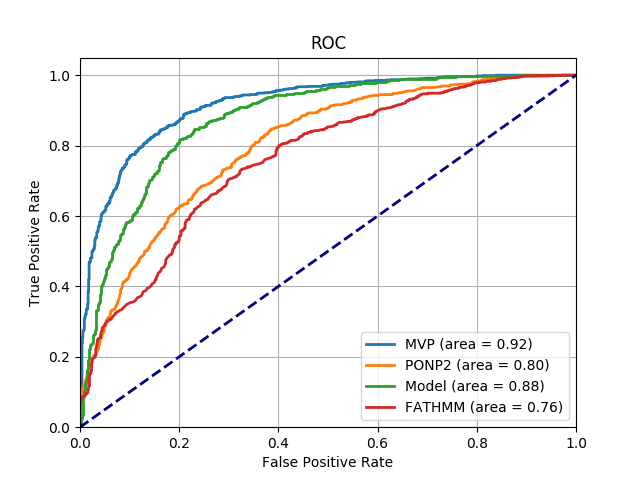
\includegraphics[width=.9\linewidth]{ALL_same_include_all_ROC.png}
  \caption{ROC}
  \label{fig:sub1_vb}
\end{subfigure}% 
\begin{subfigure}{.8\textwidth}
  \centering
  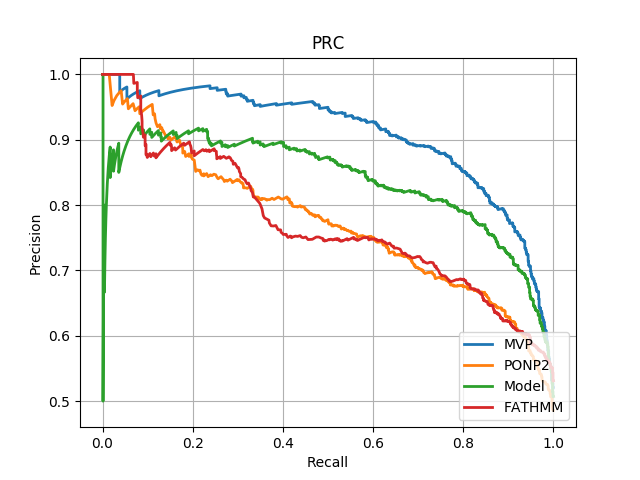
\includegraphics[width=.9\linewidth]{ALL_same_include_all_PRC.png}
  \caption{Precision-Recall}
  \label{fig:sub2_vb}
\end{subfigure}
\caption{ROC and PRC constructed from predictions on all variants in VariBench tolerance test set}
\label{fig:varibench_tolerance_roc}
\end{figure}

\subsection{HumVar \& HumDiv}

Reported performances in terms of AUC for HumVar and HumDiv found in literature\cite{wong2014snpdryad} along with those of the developed model can be seen in Table \ref{table:hum_auc}. Full metrics of the developed model can be seen in Table \ref{table:hum_metrics}. ROC curves of the developed model on both datasets can be seen in Figure \ref{fig:hum_rocs}.

For the larger HumVar dataset, the developed model achieves the highest AUC of all predictors compared, at an AUC of 0.93 on the test set.
For the smaller HumDiv dataset, the developed model achieves the second highest AUC of the predictors compared, at an AUC of 0.96 on the test set. While sensitivity and specificity are balanced for the larger HumVar dataset, the model achieves low specificity but very high sensitivity on the smaller HumDiv dataset. 

\begin{table}
\caption{Reported AUC and AUC of developed model}
\label{table:hum_auc}
\begin{center}
\begin{tabular}{lllllll}
\toprule
Predictor & AUC (HumVar) & AUC (HumDiv) \\ 
\midrule
\textbf{Developed model} & 0.93 & 0.96 \\
SNPdryad & 0.91 & 0.98   \\
PolyPhen2 & 0.89 & 0.95  \\
SIFT & 0.86 & 0.91 \\ 
MutationTaster & 0.86 & 0.90  \\ 
\bottomrule
\end{tabular}
\end{center}
\end{table}

\begin{table}
\caption{Metrics of developed model on HumVar and HumDiv datasets}
\label{table:hum_metrics}
\begin{center}
\begin{tabular}{llllllll}
\toprule
Dataset & PPV & NPV & Sens & Spec & Acc & MCC & AUC \\ 
\midrule
HumVar validation & 0.89 & 0.84 & 0.84 & 0.88 & 0.86 & 0.72 & 0.94 \\ 
HumVar test & 0.88 & 0.85 & 0.84 & 0.88 & 0.86 & 0.72 & 0.93  \\ 
HumDiv validation & 0.63 & 0.96 & 0.97 & 0.57 & 0.77 & 0.56 & 0.93  \\
HumDiv test & 0.71 & 0.96 & 0.96 & 0.71 & 0.82 & 0.68 & 0.96  \\ 
\bottomrule
\end{tabular}
\end{center}
\end{table}

\begin{figure}
\centerfloat
\begin{subfigure}{.8\textwidth}
  \centering
  \includegraphics[width=.9\linewidth]{humvar_ROC.png}
  \caption{ROC curves on HumVar}
  \label{fig:sub1_h}
\end{subfigure}% 
\begin{subfigure}{.8\textwidth}
  \centering
  \includegraphics[width=.9\linewidth]{humdiv_ROC.png}
  \caption{ROC curves on HumDiv}
  \label{fig:sub2_h}
\end{subfigure}
\caption{ROC on HumVar and HumDiv}
\label{fig:hum_rocs}
\end{figure}


\clearpage
\subsection{VariBench severity}

The reported performance for binary predictions for the VariBench severity dataset found in literature\cite{niroula2017predicting} along with the developed model's performance can be seen in Table \ref{table:severity_metrics}. These predictions classify variants into severe and nonsevere, combining the mild and moderate variants found in the dataset into nonsevere variants. The developed model has similar performance to the best performing predictor on the dataset, with an MCC of 0.21 on the independent test set. While the developed model has a higher specificity, it is less sensitive than PON-PS. ROC curves and PR curves can be seen for binary classification in Figure \ref{fig:ps_binary}. 

\begin{table}
\caption{Metrics on VariBench severity dataset}
\label{table:severity_metrics}
\begin{center}
\begin{tabular}{llllllll}
\toprule
Predictor & PPV & NPV & Sens & Spec & Acc & MCC \\
\midrule
Developed model (validation) & 0.61 & 0.62 & 0.51 & 0.71 & 0.61 & 0.23 \\
Developed model (test) & 0.67 & 0.54 & 0.53 & 0.68 & 0.61 & 0.21   \\
PON-PS (validation) & 0.49 & 0.79 & 0.66 & 0.64 & 0.65 & 0.29   \\
PON-PS (test) & 0.66 & 0.56 & 0.65 & 0.57 & 0.61 & 0.22  \\ 
MutationAssessor (validation) & 0.58 & 0.58 & 0.46 & 0.70 & 0.58 & 0.16 \\ 
MutationAssessor (test) & 0.67 & 0.45 & 0.48 & 0.64 & 0.56 & 0.12  \\ 
\bottomrule
\end{tabular}
\end{center}
\end{table}

\begin{figure}
\centerfloat
\begin{subfigure}{.8\textwidth}
  \centering
  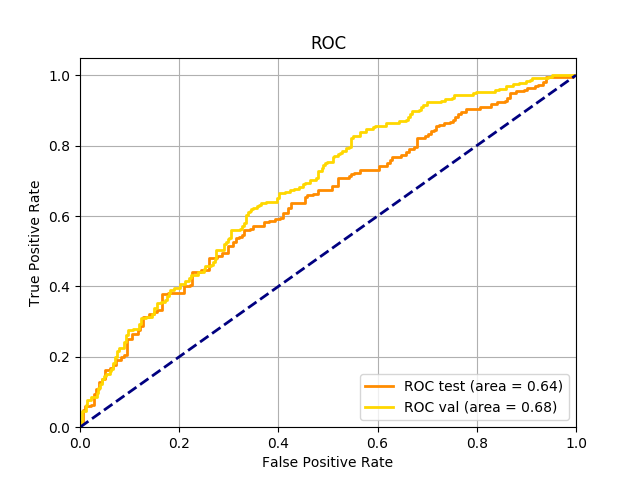
\includegraphics[width=.9\linewidth]{ps_transfer_ROC.png}
  \caption{ROC curve for binary severity classification}
  \label{fig:sub1_s}
\end{subfigure}% 
\begin{subfigure}{.8\textwidth}
  \centering
  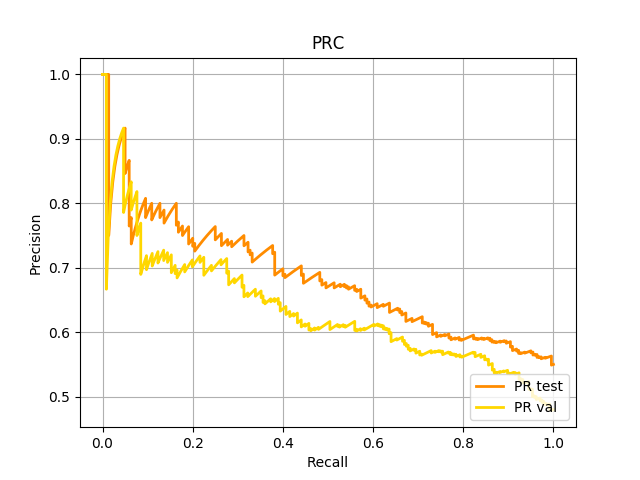
\includegraphics[width=.9\linewidth]{ps_transfer_PRC.png}
  \caption{PRC for binary severity classification}
  \label{fig:sub2_s}
\end{subfigure}
\caption{ROC and PRC for classifying variants in the VariBench severity dataset into nonsevere and severe}
\label{fig:ps_binary}
\end{figure}

The performance of the model trained and evaluated for 3-class predictions of Mild, Moderate and Severe variants can be seen as a confusion matrix in Figure \ref{fig:confmat_severity}. 

\begin{figure}
\centerfloat
\begin{subfigure}{.8\textwidth}
  \centering
  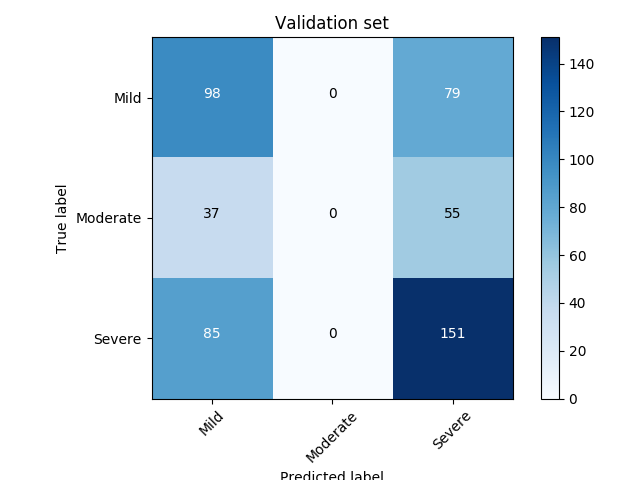
\includegraphics[width=.9\linewidth]{confmat_val_build.png}
  \caption{Validation}
  \label{fig:sub1}
\end{subfigure}% 
\begin{subfigure}{.8\textwidth}
  \centering
  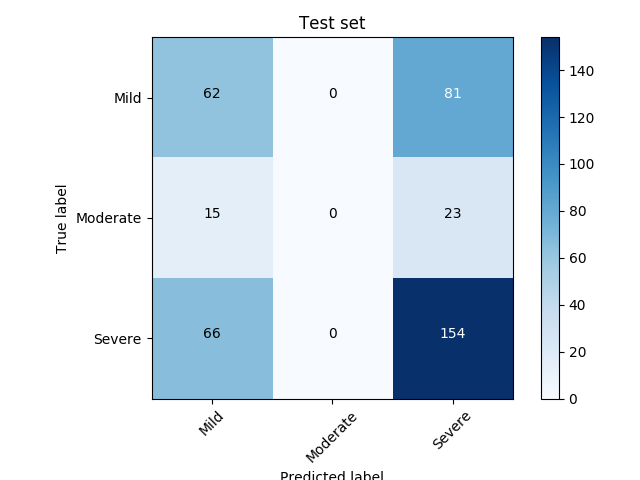
\includegraphics[width=.9\linewidth]{confmat_test_build.png}
  \caption{Test}
  \label{fig:sub2}
\end{subfigure}
\caption{Confusion matrices for training and testing on the VariBench severity dataset}
\label{fig:confmat_severity}
\end{figure}
    
    
\clearpage
\section{Discussion}

Looking at the results, the developed deep learning model has higher than state-of-the-art performance or comparable to state-of-the-art performance for all datasets. While the performance of the developed model is lower than that of MVP on the VariBench tolerance dataset, the comparison is made difficult since MVP is trained on 81\% to 90\% of variants found in the VariBench testing dataset as stated in Supplementary Tables S5 in Qi et al, 2018\cite{qi2018mvp}. This data overlap is likely also found in the auxiliary predictors used in the method, which might inflate the accuracy of the method. Data circularity at the protein level is another likely factor for the predictor or any of the auxiliary predictors, which also might inflate apparent accuracy.

General pathogenicity classification is much more accurate than severity classification, likely due to the much smaller size of the severity dataset. As can be seen in the confusion matrices in Figure \ref{fig:confmat_severity}, the model for severity prediction has difficulty distinguishing severity classes, only somewhat managing to distinguish between mild and severe variants in the validation set. The moderate variants are essentially randomly predicted as being either mild or severe. The difficulty in distinguishing moderate variants is also likely due to how the GO log-odds score is constructed, with moderate variants lumped together with mild variants when calculating reference GO term frequencies. Furthermore, it should be noted that there might be protein level data circularity due to model weights being initialized from pathogenicity prediction on the VariBench tolerance dataset, which might have some small effect on performance. It could be expected that disease severity prediction can increase in accuracy as more variants are annotated by severity in the future, but for now this remains a difficult task due to the higher difficulty of experimentally verifying and curating such data. 

Differences in dataset size is a factor in the difference in performance between the datasets, but another factor is the way the data is split. Classifying variants in proteins not seen during training does seem like a more difficult task compared to classifying variants in proteins already seen. This is likely a factor in the difference in performance between the VariBench datasets as compared to the HumDiv and HumVar datasets.

Out of all datasets, the highest AUC is reached on the HumDiv dataset, despite its smaller size. This could be due to both positive and negative examples (i.e. pathogenic and neutral) existing for every protein in the dataset. Although the performance out of all datasets was the highest on this dataset, other predictors manage to reach higher accuracies. This might be due to the smaller dataset size, not allowing the deep learning model to take full advantage of large amounts of data, or other classifier types being more suited for the task.

When evaluating different versions of the model (see Table \ref{table:model_versions}), it is clear that both information from the MSA as well as the GO terms are important, while the structural input is less important. The GO terms are likely to be important since they are the only input to capture overall protein function. That the MSA-derived input is important is very much in line with literature and existing variant effect prediction methods, since it is known that evolutionary conservation plays an important role in determining the effect of amino acid substitutions, both for disease and structure of proteins.

Compared to many other predictors, the features used as input to the developed model are relatively low level. Still, some features such as the GO-term score involve a degree of feature engineering, which ideally could be avoided using a deep learning architecture. The score is necessary in this model since it encodes information about overall protein function and characteristics, not present in the same way in only the 21-residue window. There could be other ways to encode overall protein function, on the other hand, perhaps by pre-training a network to predict overall functional class, such as if the protein is an enzyme or not. An additional issue with the current approach of using GO terms is that these already have to exist in some database, limiting the predictor to variants in already known proteins. One solution for this could be predicting the GO terms from the sequence itself, such as done by models like DeepGO\cite{kulmanov2017deepgo}. This would increase the generalization ability of the pathogenicity predictor, allowing prediction of variants in novel or unknown sequences.


\clearpage

\begin{appendices}


\newcolumntype{L}[1]{>{\raggedright\let\newline\\\arraybackslash\hspace{0pt}}m{#1}}
\newcolumntype{C}[1]{>{\centering\let\newline\\\arraybackslash\hspace{0pt}}m{#1}}
\newcolumntype{R}[1]{>{\raggedleft\let\newline\\\arraybackslash\hspace{0pt}}m{#1}}



\section{Genomic variation and protein mutations}

The human genome carries the genetic information of a person. From individual to individual, there can be a certain degree of variation in the genome, and this variation can have many consequences. Often, the variation carries with it no real functional consequence. Sometimes, the variation can be beneficial, while at other times it can be highly harmful and associated with disease.

One type of variation is single nucleotide polymorphisms, SNPs. Here, a nucleotide at a certain position in the genome is exchanged for another nucleotide. SNPs can have widely varying effects depending on where in the genome they occur. If they occur in coding regions of the genome, they can be classified into synonymous substitutions and non-synonymous substitutions. Synonymous substitutions are those substitutions that result in a codon still coding for the same amino acid, while non-synonymous substitutions cause an amino acid change in the final protein product of the coding region.\cite{gonzales2002synonymous} Through population scale sequencing, it has been estimated that individuals, when compared to a reference genome, carry around 10 000 to 11 000 non-synonymous substitutions, and 10 000 to 12 000 synonymous substitutions.\cite{10002010map} Mutations occurring in the coding regions of the genome have been found to more often be associated with disease, compared to those occurring in non-coding regions.\cite{niroula2015pon}

An amino acid substitution can have several effects on a protein. It can affect the way the protein interacts with other proteins, how it folds, as well as how it is expressed and where it is localized in the cell.\cite{reva2011predicting} These factors and others, can also cause the protein to gain a new, different function than that of its original one, or lose its function.\cite{reva2011predicting}

Mutations with experimentally verified effects can be found in literature and databases. Detailed data connecting a certain mutation and the phenotypes it gives rise to can often be found in databases specifically dedicated for the study of a certain gene or disease: locus-specific databases (LSDBs).\cite{giardine2007phencode} Efforts exist to systematically collect and organize such data into larger, wide-spanning databases. Several repositories collect large amounts of annotated variants, such as the Human Gene Mutation Database (HGMD)\cite{stenson2009human} and the Single Nucleotide Polymorphism Database (dbSNP)\cite{sherry2001dbsnp}. The database VariBench\cite{nair2013varibench} collects and organizes variants from databases such as dbSNP into benchmark datasets, containing both positive and negative samples (i.e. variants having a certain effect and variants not having an effect). It contains datasets related to protein tolerance (whether variants are benign or not), protein stability, mismatch repair gene variation, protein mutations affecting transcription factor binding, as well as splice site variation.\cite{nair2013varibench} These datasets are useful for developing and assessing prediction tools intended for use in these domains. The sizes of these datasets vary, but the largest of these contains up to 19 000 pathogenic non-synonymous SNPs and 21 000 neutral non-synonymous SNPs.

\section{Predicting the effect of mutations}

\subsection{Variant effect predictors}

For predicting the effect of non-synonymous SNPs leading to protein mutations, a number of predictive tools have been developed. The meta-database OMICtools\cite{henry2014omictools} lists over 130 variant effect prediction tools, many of them made for predicting effects of amino acid substitutions. A collection of several such tools can be seen in Table \ref{table:predictors} on page \pageref{table:predictors}. The table describes tools in terms of what kinds of features in the input data the classifier looks at, what type of classifier the tool uses, what data the classifier is trained on if it is a machine learning approach, as well as general notes on the tool.

Some tools are specialized for certain types of variants, such as VEST\cite{carter2013identifying} for Mendelian disease mutations or PON-MMR2\cite{niroula2015classification} for variants in mismatch repair proteins.

Many of these tools employ some form of machine learning to train a predictor on a certain dataset, which then allows the predictor to generate a prediction on a novel mutation, given some input data. Others develop some form of rule or mathematical operation to calculate a score, which is then used to classify a variant. 

The performance of available predictors differs somewhat depending on what dataset they have been trained and tested on. Proper comparison of the performance of available predictors is made somewhat complicated since many have not been trained and tested on standard benchmark datasets. If such predictors are then evaluated on a standard test dataset, their performance can be biased due to overlap between datasets. Evaluations carried out using fully disjoint datasets found that the performance measures of most tools greatly decreased from their reported performance.\cite{grimm2015evaluation} Some bias is also introduced at a protein level, if variants from the same protein are present in training and testing datasets.\cite{grimm2015evaluation} However, some of the best performing predictors have taken care to avoid any such data circularity, and report classification accuracy up to 77\% with a Matthews correlation coefficient (MCC) of 0.53\cite{niroula2016variation} when classifying variants into pathogenic and neutral.


\subsection{Sequence information and features}

What most predictors have in common, especially those with good performance, is that they utilize information obtained from a multiple sequence alignment (MSA) of homologous protein sequences.\cite{miosge2015comparison} A homologous sequence (in terms of DNA or amino acids), is a sequence that has a statistically significant similarity to some reference sequence, which indicates common ancestry between the sequences.\cite{pearson2013introduction} Homologous sequences can further be divided into paralogs and orthologs, where paralogs arise from duplication of a gene within a genome, and orthologs arise from speciation events. While many variant effect predictors include all homologous sequences, certain predictive tools such as SNPdryad\cite{wong2014snpdryad} find that excluding paralogous sequences and only including orthologuous sequences in an MSA can improve classification accuracy.

Homologous sequences can be found by comparing a query sequence against a large database of other sequences, and evaluating similarity through some scoring scheme. One of the most common ways of doing this is by using BLAST\cite{altschul1990basic}, but can also more recently be done by using hidden Markov model (HMM) based approaches with programs like HMMER.\cite{eddy2009new}

The MSA built from homologous sequences can be used to calculate statistics indicating evolutionary conservation. For example, an MSA of homologous protein sequences can be used to infer how important a certain residue at a certain position is for maintaining function and structure of a protein.\cite{valdar2002scoring} An example of an MSA can be seen in Figure \ref{fig:msa}. If some position in an alignment of many similar proteins always seems to contain a certain amino acid, it is likely that the amino acid at that position is important for the protein function in some way. Scoring such conservation can be done in many different ways, but is often done by calculating some version of an entropy score, such as Shannon's entropy for a column in the MSA\cite{valdar2002scoring}:

\begin{equation}
S = -\sum_{i}^{K} p_i \log_2 p_i
\end{equation}

where $p_i$ is the fractional frequency of an amino acid of type \textit{i} out of \textit{K} types.

\begin{figure}
  \centering
  \hspace*{-0.8in}
  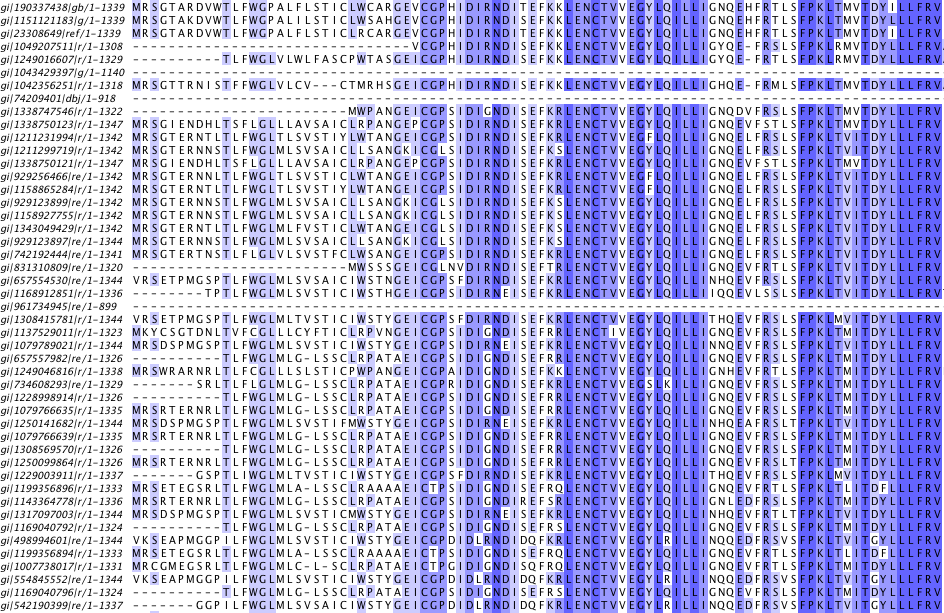
\includegraphics[scale=0.5]
    {msa_example_edited.png}
  \centering
  \caption{ MSA of protein sequences. Blue columns indicate more conserved positions. }
  \label{fig:msa}
\end{figure}


Certain predictors also use information about the structure of the protein of interest. This information can for instance determine if an amino acid substitution occurs in the hydrophobic protein core, or if it has an effect on electrostatic interactions or other interactions.\cite{adzhubei2013predicting} Other predictors include information about the physical and chemical properties of the amino acids involved in the mutation, and around the mutation site.\cite{niroula2017predicting}

\clearpage
\begin{center}
\setlength\LTleft{-1.2in}
%\setlength\LTright{-1in}
\begin{small}
\begin{longtable}{| l | L{4cm} | L{2cm} | L{3cm} | L{5cm} |}
\caption{Variant effect predictors able to handle amino acid substitutions.\\Abbreviations: AA (amino acid), RF (random forest), GO (gene ontology), MSA (multiple sequence alignment), SVM (support vector machine)}
\label{table:predictors}
\endfirsthead
\endhead
\hline
Predictor & Features & Classifier type & Training dataset & Notes \\ \hline
PON-P2 & Evolutionary conservation, physical and biochemical properties of AAs, GO annotations & RF & VariBench PON-P2 & Classifies into pathogenic/neutral/unknown.  \\ \hline
PON-MMR2 & Similar to PON-P2 & RF & VariBench PON-MMR & Specialized for mismatch repair proteins. Classifies into pathogenic/neutral. \\ \hline
PON-PS & Similar to PON-P2 & RF & VariBench PON-PS & Predicts severity of AA substitutions. Classifies into severe and nonsevere. \\ \hline
MutationAssessor & Functional impact score based on evolutionary information & Score threshold &  N/A & Specialized for cancer genomics. \\ \hline
SIFT & Scaled probabilities of AAs in positions in MSA & Score threshold & N/A & MSA created from homologs found with BLAST. Classifies into tolerated/deleterious. \\ \hline
PolyPhen-2 & Features from sequence annotations, MSA, 3D structures & Naive Bayes & HumDiv / HumVar (compiled from variants in UniProtKB) & Calculates the posterior probability that a mutation is damaging. \\ \hline
PROVEAN & Differences in E-value from BLAST & Score threshold & N/A & Uses delta score (function of change in alignment score because of a substitution). Can handle several simultaneous substitutions in a protein. \\ \hline
MutationTaster2 & Regulatory features from Ensembl, evolutionary conservation scores of nucleotides & Bayes classifier  & Polymorphisms from 1000G, mutations from HGMD & Starts from DNA sequence; can also handle synonymous substitutions. \\ \hline
VEST & Features from SNVBox & RF & Mutations from HGMD and variants from the Exome Sequencing Project & Specialized for mendelian disease mutations. \\ \hline
CADD & Annotations from Ensembl VEP and scores from other programs & SVM & Simulated variants and variants from ClinVar & Combines annotations and scores from many different programs. \\ \hline
FATHMM & AA probabilities in a HMM & Score threshold & N/A & The HMM is constructed from an MSA obtained with JackHMMER. \\ \hline
PMUT & Features from internal databases, structural features, features from MSA & Shallow neural network & Not specified & Outputs a pathogenicity index ranging from 0 to 1. \\ \hline
PantherPSEP & Evolutionary score from MSA & Score threshold & HumVar & Obtains alignments from PANTHER database. \\ \hline
MAPP & Score based on MSA and physiochemical properties of AAs & Score threshold & N/A & Classifies into neutral/moderately deleterious/strongly deleterious. \\ \hline
Align-GVGD & Grantham variation and difference of a position in MSA & Score threshold & N/A & Grantham analysis is based on physiochemical characteristics of amino acids. \\ \hline
DANN & Same as CADD & Neural network & Same as CADD & Network structure:
input layer, sigmoid output layer, three 1000-node tanh hidden layers. \\ \hline
Condel & Combines predictions from Logre, MAPP, MutationAssessor, PolyPhen-2, SIFT & N/A & N/A & Consensus tool. \\ \hline
SNPdryad & Features from MSA of orthologous proteins, physiochemical properties of AAs & RF & HumDiv and HumVar & Found that excluding paralogs leads to better performance. \\ \hline
SNAP2 & Wide range of amino acid properties, explicit sequence, PSIC profiles, various structural properties, residue flexibility, various annotations, contact potentials & 10 different shallow neural networks  & Variants from PMD, SWISS-PROT, OMIM, HumVar & Uses a very wide range of features. Classifies into effect/neutral. \\ \hline
\end{longtable}
\end{small}
\end{center}
\clearpage

\section{Machine learning}

\subsection{Conventional methods}
As can be seen in Table \ref{table:predictors}, the vast majority of tools based on machine learning are conventional machine learning approaches. In this approach, feature engineering is done on the input data to extract feature vectors which are then fed into some classifier. Some common classifier types for variant effect prediction are Random Forest (RF) classifiers, Support Vector Machine (SVM) classifiers, and some more simple probabilistic classifiers such as the Naive Bayes classifier.

\subsection{Feature engineering and selection}
The feature engineering in many of the tools can be quite involved. Often, it requires collecting data from many different sources and running what can sometimes be computationally expensive steps. For example, a very informative feature is codon-level selective pressure\cite{niroula2015classification}, but it requires collecting a protein's corresponding cDNA sequence, aligning codons, and computing on the alignment. This computational expense can be alleviated somewhat though, by using pre-computed feature vectors when making predictions.

When having a large feature set, feature selection is also a step that has to be done for most machine learning approaches. This can involve methods ranging from simple filter methods to more computationally expensive wrapper methods such as forward feature selection.

\section{Deep learning}

\subsection{Problem domains}

Some of the more recent tools in Table \ref{table:predictors} are based on neural networks, some with several hidden layers. As of yet, though, they are mostly shallow densely connected feedforward networks using similar (or the same in one case) features as more conventional tools. One advantage of deep learning approaches is that it allows for an end-to-end feature extraction and classification model based on lower level representations of input data.

Deep learning methods have recently shown promise in many other applications of predicting properties of proteins. Deep learning shows success in protein contact prediction\cite{skwark2014improved}, and for assessing protein model quality, a Multilayer Perceptron (MLP) achieves state-of-the-art results.\cite{uziela2017proq3d} 

More complex architectures can be found in other problem domains. DeepCNF\cite{wang2016protein} utilizes a deep convolutional neural network (CNN) combined with conditional neural fields\cite{peng2009conditional} to predict the secondary structure of a protein. It does this using only a sparsely encoded amino acid sequence and a position specific scoring matrix (PSSM) obtained from an MSA as input.

For some problem domains, an encoding of only the protein sequence itself is used as input to deep models. This has been used to predict protein function in a model using a Recurrent Neural Network (RNN), containing long-short-term-memory (LSTM) units.\cite{liu2017deep} Another model predicts enzyme function with a network combining both CNN and RNN components.\cite{li2017deepre} Using only a sequence might not be enough information input for a problem heavily dependent on evolutionary information, however.

\subsection{Multilayer perceptrons}

One of the most simple types of deep neural networks are MLPs. Some of the predictors in Table \ref{table:predictors} belong to this class of network. MLPs consist of an input layer, an output layer, and a number of hidden layers in between. Each layer consists of a number of neurons, or nodes. Nodes are connected in a feedforward fashion with a weight parameter for each connection. Each node computes an output from an activation function involving its connections and their weights, as well as a bias. This computation can be described for some activation function \textit{f}, weight vector \textbf{w}, input vector \textbf{x} and bias \textit{b} as follows:

\begin{equation}
y = f(\mathbf{w}^T\mathbf{x} + b)
\end{equation}

Often used activation functions include the logistic sigmoid function

\begin{equation}
\sigma(x) = \frac{1}{1 + e^{-x}}  
\end{equation}

or the activation function used in a rectified linear unit (ReLU)

\begin{equation}
f(x) = \textrm{max}(0,x)  
\end{equation}

By stacking several layers of such nodes in a network, the network becomes capable of approximating non-linear functions. For a given set of input and output data, network parameters can be adjusted in a supervised fashion. This allows the network to capture relationships between input features and be used for classification problems. Network parameters are adjusted using some form of loss function such as the mean squared error (MSE) or the cross-entropy loss between network output and desired output, along with a gradient-based optimization algorithm. For computing the gradient on which to base a parameter update, back-propagation is used. For updating the parameters, several optimization algorithms exist such as stochastic gradient descent (SGD) or more recent variants thereof such as Adam.\cite{kingma2014adam}

\subsection{Convolutional networks}

Convolutional neural networks share some similarities to the multilayer perceptrons described above. It is a feedforward network, uses similar activations, and is trained in the manner described above. However, a convolutional network makes use of sparse connectivity by only connecting neurons in a hidden layer to a certain region of input, and sliding this region across the input space. Additionally, instead of using individual weights and biases for each neuron, neurons share parameters, defining a filter. A convolutional layer will then consist of a number of such filters. Typically, a convolutional network will also make use of so-called pooling layers applied on the feature maps created by convolutional layers, to create a more condensed version of these.
An example of a convolutional network can be seen in Figure \ref{fig:deepsf}, applied to protein sequence derived input.

\begin{figure}
  \centering
  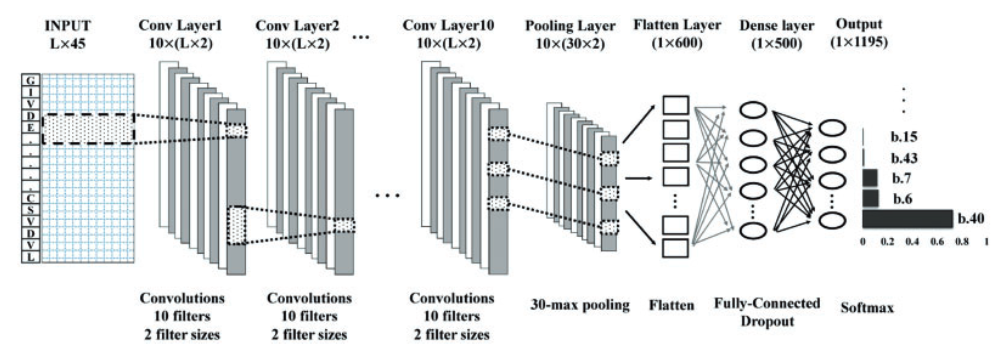
\includegraphics[scale=0.4]
    {DeepSF_model_2.png}
  \centering
  \caption{ 1D deep convolutional network used in DeepSF. Reproduced from Hou et al, 2017.\cite{hou2017deepsf} }
  \label{fig:deepsf}
\end{figure}

While not widely used for variant effect prediction problems, convolutional networks have shown remarkable success in other protein prediction domains. One state-of-the-art model for contact prediction\cite{wang2017accurate} uses residual neural network blocks with first 1-dimensional and then 2-dimensional convolutions, using MSA-derived features and some other protein features as input. The structure of the network allows it to handle proteins of varying length. Similar input features are used in another model combining six CNNs, also for contact prediction.\cite{adhikari2017dncon2} Other examples of 1-dimensional CNN models applied to protein sequences are Must-CNN, used for structural prediction\cite{lin2016must} and DeepSF, for mapping protein sequences to folds.\cite{hou2017deepsf} Going beyond those problems based on protein sequences, CNNs have been used to predict effects of non-coding variants in DNA sequences.\cite{zhou2015predicting}

A 1D convolutional layer can learn to recognize local patterns in a sequence, and these patterns can then be recognized at other locations in the sequence. 2D layers have such properties for local patches in a matrix. These local patterns are able to capture important relationships between, for example, amino acids in a sequence.







\clearpage
\bibliographystyle{unsrtnat}
\bibliography{ref}

\end{appendices}

\newpage
\mbox{}
\newpage

\includepdf[pages={2}]{omslag_baksida.pdf}

\end{document}





